\documentclass[uplatex]{jsarticle}
\usepackage{nidanfloat}
\usepackage[dvipdfmx]{graphicx}
\usepackage[dvipdfmx]{color}
\usepackage{amsmath}
\newcommand{\argmax}{\mathop{\rm arg~max}\limits}
\newcommand{\argmin}{\mathop{\rm arg~min}\limits}
\title{レビューデータ分析におけるトピック抽出モデルに感情の要素と文脈を考慮した単語分散表現モデルであるBERTを導入したモデルの拡張\\「Topic Sentiment Joint Model with Word embeddings BERT」}
\author{東北大学 経済学研究科 C0EM1023 長谷川 一旗}
\date{\today}
\begin{document}
\maketitle

%概要
\begin{abstract}
    \large
    マーケティングにおいて、オンライン上に散見されるレビュー文から、消費者の商品に対する感情や消費者がどのような点に関心を持っているかについて分析することは非常に重要視されている。
    したがって、テキストから書き手の感情を分析する感情分析やテキストからトピックと呼ばれる書き手の関心事を抽出するトピックモデルといった手法は、近年の主要な研究分野になっており、組み合わせたモデルが登場するなど研究が盛んになっている。
    加えて、こうした感情分析やトピックモデルに対して、単語の分散表現と呼ばれる今までのBag-of-wordsより柔軟な言語表現を導入することで、性能や精度の向上を目指したモデルも存在してきている。
    しかしながら、これら自然言語処理分野においてbag-of-wordsなどに代表される言語表現において、文脈を考慮することのできないという点が問題視されていた。
    その問題点を解決したBERTという文脈を考慮した単語分散表現の獲得に成功したモデルの登場により、自然言語処理分野では近年大きな変化を遂げている。
    したがって、本研究では感情分析とトピックモデルを組み合わせたモデルに対して、BERTから得られた文脈を考慮した単語分散表現を導入することで、感情分析の精度やトピック抽出での意味的結束性の向上が見られるかを検証していく。
\end{abstract}
\newpage
\tableofcontents
\twocolumn
\section{Introduction}
高度な情報化社会の成立により、テキストデータが急速に蓄積されつつある現代社会において、テキストから隠れた知見を発見するためのテキストマイニングは非常に多くの分野で活用されている。

マーケティング分野においては、Eコマース事業やソーシャルメディアの急速な発展に伴って、オンライン上に散見されるレビューを分析し、消費者の感情やトピックを抽出し理解することが、企業にとって非常に重要視されつつある。
したがって、テキストから書き手の感情を解析する手法やテキストから書き手の関心ごとであるトピックを抽出するトピックモデルといった手法は、その重要性から近年の主要な研究分野の一つとなっており、様々な改良モデルが考案されている。
Joint Sentiment Topic Model(JST)\cite{JST}では、Latent Dirichlet Allocation(LDA)\cite{LDA}にセンチメント層を導入することで、テキストから感情とトピックを同時に抽出することを可能にし、より実用的なモデルへと拡張している。
Gaussian LDA for Topic Models with Word Embeddings\cite{Gaussian LDA}では、自然言語処理分野において、分散表現(Word Embeddings)と呼ばれる単語を高次元のベクトルで表現する技術をLDAに導入することで、意味的に近く解釈のしやすいトピックの
抽出が可能となったと同時にモデルの性能の向上も示されている。Joint Sentiment Topic Model(JST)では、学習コーパスの少ない場合にモデル性能の低下することが問題として指摘されており、この問題点の解決するために分散表現を導入したTopic Sentiment Joint Model with Word Embeddings\cite{TSWE}というモデルも存在する。
このモデルでは、外部の大規模コーパスを用いた分散表現の導入によって、モデルの性能が大幅に向上したことが示されている。しかしながら、これらのモデルに利用されている分散表現は、Word2Vec\cite{Word2Vec}という文脈を考慮していない分散表現である。文脈を考慮しない分散表現では、異なる意味合いを持つ単語に対して
それぞれの意味を区別できない分散表現になってしまうため、多義語のある文章に対して十分な性能を発揮できないという問題点が指摘されている。近年の自然言語処理分野では、こうした問題点に対応するために深層学習を利用することで文脈を考慮した単語分散表現の獲得を目指す研究が盛んに行われており、ELMo\cite{ELMo}やBERT\cite{BERT}といったモデルは
既存の分散表現モデルと比較して、高い性能を誇ることが知られている。よって、既存の分散表現であるWord2Vecを利用している様々なタスクやモデルにおいて、こうした文脈を考慮した分散表現を置換してあげることにより性能の向上が見込まれるが、それらを検証した論文は多くは出てきていません。

したがって、本稿では分散表現を利用したセンチメントとトピックの同時抽出モデルであるTopic Sentiment Joint Model with Word Embeddings(TSWE)に導入する分散表現として、文脈考慮型の分散表現を導入したモデルを提案し、その有効性について実験を通して検証を行っていく。

%先行研究
\section{Related Researches}
%LDA
\subsection{Latent Dirichlet Allocation(LDA)}
LDAは、Bleiら\cite{LDA}によって提案された文書の確率的生成モデルである。LDAでは、文書には複数のトピックが存在すると仮定し、文書中に含まれる単語にトピックを割り当てる。トピックは、文書から観測できないため、文書内の単語の共起情報からトピックを推定する。
図1(a)に示すLDAの生成過程をまとめると以下の通りである。
\begin{enumerate}
    \item for $k=1$ to $K$
          \begin{enumerate}
              \item Draw word distribution $\phi_{k} \sim $Dir($\beta$)
          \end{enumerate}
    \item For each document $d$
          \begin{enumerate}
              \item Draw a topic distribution $\theta_{d} \sim $Dir($\alpha$)
              \item For each word index n from 1 to $N_{d}$
                    \begin{enumerate}
                        \item Draw a topic $z_{dn} \sim$ Multi($\theta_{d}$)
                        \item Draw a word $w_{dn} \sim$ Multi($\phi_{z_{dn}}$)
                    \end{enumerate}
          \end{enumerate}
\end{enumerate}

LDAは、自然言語処理分野だけでなく多種多様な分野に応用可能なモデルであり、改良も容易であることから様々な改良モデルが存在する。その中でも、センチメント層を導入することで感情推定とトピック推定を同時に行うことを可能にしたモデルであるJST\cite{JST}モデルを2.2節、分散表現を導入することでその性能を向上させただけでなく、未知語に対しても対応可能になっているGaussian LDA\cite{Gaussian LDA}モデルを2.3節で紹介する。
2.4節では、本稿での提案手法の基礎にもなったJSTモデルに分散表現を導入することで、より性能を向上させたTSWE\cite{TSWE}モデルの紹介を行う。
% JST
\subsection{Joint Sentiment/Topic Model for Sentiment Analysis(JST)}
JSTは、Linら\cite{JST}によって提案された文書からセンチメントとトピックの抽出を目的としたモデルである。JSTでは、文書単位での感情分類を達成するために、文書層とトピック層との間にセンチメント層を導入することで通常のLDAモデルを拡張した。
JSTでは、従来のLDAと異なり、$S$個のセンチメントラベルが文書と紐づけられており、そのもとでトピックがセンチメントラベルに紐づけられている。したがって、単語はセンチメントラベルとトピックの両方に紐づけられることになる。
図1(b)に示すJSTの生成過程をまとめると以下の通りである。
\begin{enumerate}
    \item For each topic-sentiment pair ($k$,$l$)
          \begin{enumerate}
              \item Draw word distribution $\phi_{k,l} \sim $ Dir($\beta$)
          \end{enumerate}
    \item For each document $d$
          \begin{enumerate}
              \item Draw a sentiment distribution $\pi_{d} \sim $ Dir($\gamma$)
              \item For $l=1$ to $S$
                    \begin{enumerate}
                        \item Draw a topic distribution $ \theta_{d,l} \sim $ Dir($\alpha$)
                    \end{enumerate}
              \item For each word index n from 1 to $N_{d}$
                    \begin{enumerate}
                        \item Draw a sentiment label $l_{dn} \sim \pi_{d}$
                        \item Draw a topic $z_{dn} \sim \theta_{d, l_{dn}}$
                        \item Draw a word $w_{dn} \sim \phi_{z_{dn},l_{dn}}$
                    \end{enumerate}
          \end{enumerate}
\end{enumerate}

映画のレビューデータセットを利用した評価実験では、他のラベル付きアプローチと比較して、文書レベルでの感情分類において非常に優れた性能を示している。加えて、抽出されたトピックからは確かに一貫したトピックとなっていることも示している。
しかしながら、このモデルでは単語をBag-of-wordsとして表現しているため、単語の順序を考慮出来ていないということが指摘されている。

%Gaussian LDA
\subsection{Gaussian LDA for Topic Models with Word Embeddings}
分散表現学習の登場により、トピックモデルと分散表現を組み合わせ、より意味的に一貫したトピックが生成されやすくなることを目指した研究が、Gaussian LDA\cite{Gaussian LDA}である。
このモデルは、Huら\cite{Gaussian}が提案したLDAにおけるトピックを生成する分布を多次元ガウス分布にするというモデルに単語の分散表現を組み合わせたもので、Dasら\cite{Gaussian LDA}によって提案された。連続空間上に埋め込まれた単語ベクトル
に対して、トピック$k$を同一空間上での多次元ガウス分布とした。これによって、トピック毎の単語分布が連続分布となり、この分布から単語ベクトルが生成される過程がモデル化されている。
図1(c)に示すGaussian LDAの生成過程をまとめると以下の通りである。

\begin{enumerate}
    \item for $k=1$ to $K$
          \begin{enumerate}
              \item Draw topic covariance $\bf{\Sigma_{k}} \sim \mathcal{W}^{-1}(\Psi, \nu)$
              \item Draw topic mean $\bf{\mu_{k}} \sim \mathcal{N}(\bf{\mu}, \frac{1}{\mathcal{K}}\bf{\Sigma_{k}})$
          \end{enumerate}
    \item For each document $d$
          \begin{enumerate}
              \item Draw a topic distribution $\theta_{d} \sim $Dir($\alpha$)
              \item For each word index n from 1 to $N_{d}$
                    \begin{enumerate}
                        \item Draw a topic $z_{dn} \sim$ Categorical($\theta_{d}$)
                        \item Draw $v_{dn} \sim \mathcal{N}(\bf{\mu_{z_{dn}}}, \bf{\Sigma_{z_{dn}}})$
                    \end{enumerate}
          \end{enumerate}
\end{enumerate}

このモデルでは、従来のLDAと異なり単語をBag-og-wordsとして表現するのではなく、分散表現を用いて表現することで、分散表現が類似しているつまり意味的に近しいと思われる単語を同じトピックに割り当てやすくなり、トピック内の意味的統一性が向上し、自己相互情報量(PMI)も上昇することが報告されている。
しかしながら、このモデルで利用されている分散表現はWord2Vec\cite{Word2Vec}と呼ばれる手法を用いて作成されたものである。この手法では、Bag-of-wordsと同じく単語の順序を考慮できていないため、文脈を考慮した結果にならず多義語などの場合に推定がうまくできない可能性が残されている。

\begin{figure*}
    \begin{tabular}{ccc}
        \begin{minipage}[b]{0.33\hsize}
            \begin{center}
                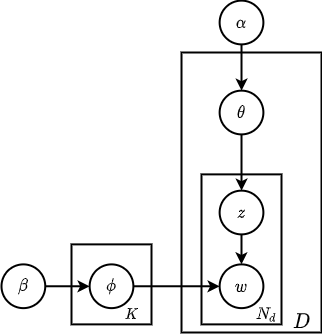
\includegraphics[width=4cm]{picture/LDA.png}
                (a)LDA
            \end{center}
        \end{minipage}
        \begin{minipage}[b]{0.33\hsize}
            \begin{center}
                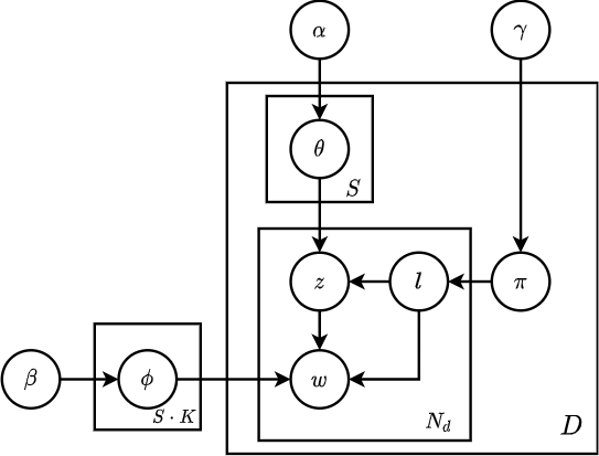
\includegraphics[width=5cm]{picture/JST.png}
                (b)JST
            \end{center}
        \end{minipage}
        \begin{minipage}[b]{0.33\hsize}
            \begin{center}
                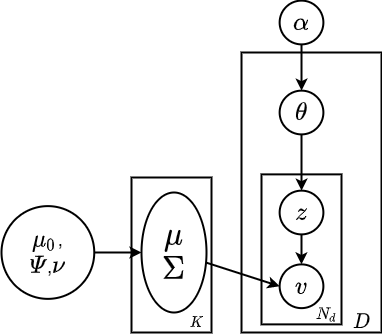
\includegraphics[width=4cm]{picture/GaussianLDA.png}
                (c)Gaussian LDA
            \end{center}
        \end{minipage}
    \end{tabular}
    \caption{グラフィカルモデル}
\end{figure*}

%TSWE
\subsection{Topic and Sentiment Model with Word Embeddings(TSWE)}
TSWEは、JSTに外部の大規模コーパスから学習させた分散表現を導入したJoint Topic Sentiment Modelで、Fuら\cite{TSWE}によって提案されたモデルである。
TSWEでは、学習コーパスが短く小さい場合に、それまでのTopic Sentiment Joint Modelで問題視されていた、単語の共起情報を使用することによって生じる分布の推定がうまくいかない問題を単語の分散表現を導入することにより解決を試みた研究である。
TSWEでは、JSTにおけるディリクレ多項式成分をSentiment-Topic-Wordのディリクレ多項式成分とWord Embeddings成分の混合成分に置換している。
このモデルでは、Word Embeddings成分から単語を生成する確率を以下のように定めている。
\begin{equation}
    MulT(w_{i}|\nu_{k}\omega^{\mathrm{T}}) = \frac{{\rm exp}(\nu_{k}\omega_{w_{i}})}{\Sigma_{w_{i}^{'}\in{W}}{\rm exp}(\nu_{k}\omega_{w_{i}^{'}})}
\end{equation}

図2に示すTSWEの生成過程をまとめると以下の通りである。

\begin{enumerate}
    \item For each topic-sentiment pair ($l$,$k$)
          \begin{enumerate}
              \item Genearte the word distribution of the sentiment-topic pair $\phi_{l,k} \sim $ Dir($\beta$)
          \end{enumerate}
    \item For each document $d$
          \begin{enumerate}
              \item Draw a distribution $\pi_{d} \sim $ Dir($\gamma$)
              \item For $l=1$ to $S$ under document $d$
                    \begin{enumerate}
                        \item Draw a topic distribution \\ $ \theta_{d,l} \sim $ Dir($\alpha$)
                    \end{enumerate}
              \item For each word index n from 1 to $N_{d}$
                    \begin{enumerate}
                        \item Draw a sentiment label \\ $ l_{dn}  \sim$ Multi($\pi_{d}$)
                        \item Draw a topic $z_{dn} \sim $ Multi($\theta_{d, l_{dn}}$)
                        \item Draw a binary indicator variable \\ $s_{dn} \sim $ Ber($\lambda$)
                        \item Draw a word \\$w_{dn}  \sim (1-s_{dn})$Multi$(\phi_{z_{dn},l_{dn}})+(1 - s_{dn})MulT(\nu_{z_{dn}}\omega^{\mathrm{T}}$)
                    \end{enumerate}
          \end{enumerate}
\end{enumerate}

しかしながら、このモデルでもGaussian LDA\cite{Gaussian LDA}同様、分散表現としてWord2Vec\cite{Word2Vec}で学習させた分散表現を用いており、依然として文脈を考慮できないという問題点が残されている。
本研究では、この問題点を解決するために利用する分散表現をBERT\cite{BERT}と呼ばれる手法で学習させた文脈を考慮できる分散表現を用いて、その性能の向上を図る。
こうした点を踏まえ、次節以降では、単語分散表現を獲得する手法として有名なWord2Vec\cite{Word2Vec}や文脈考慮型分散表現の作成をはじめて可能にしたELMo\cite{ELMo}、そのELMoの性能を大幅に向上させただけでなく、汎化性能をも高めたBERT\cite{BERT}について基本的な概念を説明していく。

\begin{figure}[thp]
    \begin{center}
        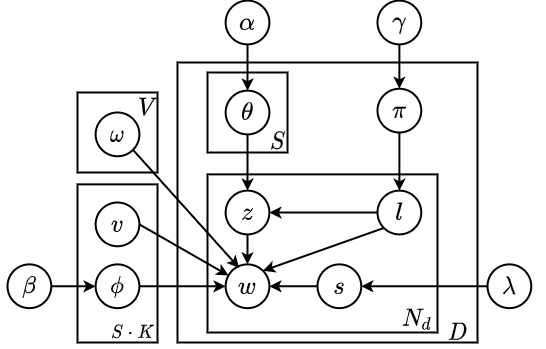
\includegraphics[width=6cm]{picture/TSWE.png}
    \end{center}
    \caption{TSWEのグラフィカルモデル}
\end{figure}
%図の作成or差し替え
\begin{figure}[tbp]
    \begin{center}
        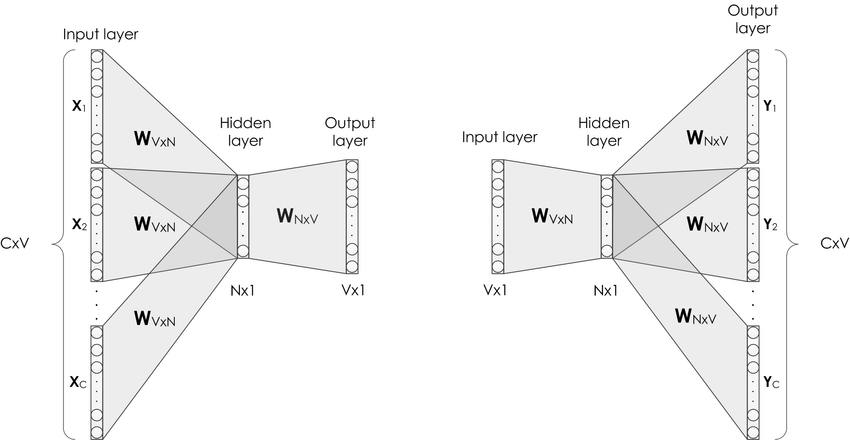
\includegraphics[width=6cm]{picture/Word2Vec.png}
    \end{center}
    \caption{Word2VecにおけるCBOWモデル(左)とSkip-gramモデル(右)\protect\footnotemark[1]}
\end{figure}
\footnotetext[1]{Tutubalinaら\cite{Graph}より引用}


%分散表現の関連研究 Appendixに回すかも
\subsection{Word2Vec}
Word2Vecは、Mikolovら\cite{Word2Vec}が提案したニューラルネットワークを用いて、単語の分布表現を獲得する手法である。つまりは単語を低次元の密なベクトルで表現したものを学習する手法である。
従来、自然言語処理のタスクではテキストデータを扱う際に、bag-of-wordsやLSI\cite{LSI}、pLSI\cite{pLSI}で圧縮したベクトルを用いてきた。しかしながら、これらの手法は次元数が高次元になってしまい計算効率が悪くなってしまう問題点や圧縮した際の精度的な問題点が残されてしまっていた。
こうした問題を解決するため、Mikolovらは単語の意味は単語の周辺の単語によって決定されるという分布仮説の下、テキスト中の各単語を周辺単語から予測するというタスクを設定し、このタスクを大規模なテキストデータからニューラルネットワークによって学習させることで各単語に対する概念ベクトルを獲得した。
Word2Vecには、図3左で示される、周辺の単語から対象とする単語が現れる確率を最大するように学習させる、Countinous Bag-of-Words(CBOW)と呼ばれる手法と図3右で示される、対象の単語を入力とした際の周辺の単語予測のエラー率が最小になるように学習させる、Skip-gramという手法が存在するが、どちらにせよ最終的に単語の分布表現が生成される。
これにより、単語を意味空間上に対応させることができ、意味的に近い単語の分類や単語を意味的に計算することが可能になった。

しかしながら、この手法では対象とする単語とその周辺にどのような単語が存在するかという点しか考慮できず、語順によって異なる意味に捉えられるような単語をうまく表現できないという問題点がある。

コンピュータの計算能力の向上に伴い、深層学習という多層なニューラルネットワークの学習が容易になったことを受け、自然言語処理分野でも凄まじい発展が見られた。
次節で紹介する深層学習を用いた分散表現を獲得する手法を紹介する。

\subsection{ELMo}
ELMoは、Matthewら\cite{ELMo}によって提案された、深層学習を用いることで文脈を考慮した単語の分散表現を獲得する手法である。
ELMoは、LSTM\cite{LSTM}と呼ばれる時系列データを学習することのできるリカレント・ニューラルネットワーク(RNN)の一種を用いた、多層の双方向LSTMによる単語レベルの言語モデルである。
Word2Vecと同様に対象単語の予測確率が高くなるように学習させる点は変わらないが、文頭から対象単語までの順方向と文末から対象単語までの逆方向という双方向の情報を用いて予測させている点がELMoの特徴になっている。
これにより、今まで考慮出来ていなかった文脈を踏まえた分散表現の獲得に成功したのである。加えて、ELMoでは、双方向型言語モデルの中間層によって単語を表現していることも注目すべき点である。

しかしながら、厳密な双方向言語モデルにおいては、予測する単語の先の単語、例えば順方向の場合は対象単語から文末までの単語を事前に知っていることになる。これは、予測においては事前に答えを知っている状態に当たるためうまく予測モデルを作成できないという問題点が生じる。
この問題を解決するために、ELMoでは順方向の情報を用いたモデルと逆方向の情報を用いたモデルを別々に学習させた後、統合する手法が採用されているが、この別々にモデルを学習させている点が浅い双方向モデルと呼ばれ、実際に文脈を捉えているか疑問視されている点でもある。
図4にグラフィカルモデルを示す。

\subsection{BERT}
BERTは、Devlinら\cite{BERT}によって提案された、Transformer\cite{Transformer}という深層学習の手法を用いた様々な自然言語処理タスクに応用可能な事前学習モデルである。
BERTでは、Masked Language Model(MLM)とNext Sentence Prediction(NSP)という二つのタスクを用いて学習させることで、双方向言語モデルにおける学習時に予測対象の先の単語が見えてはいけないという制約を克服した。
MLMは、入力文における15\%の単語に対し、確率的に3つの処理を施した状態でその処理を行う前の単語を予測させるというタスクである。
3つの処理とは、選択された15\%のうち、80\%を[MASK]に置換するマスク変換処理、10\%を別単語に置換する処理、そして残りの10\%は何もせずそのままにする処理となっている。これによって、単語レベルでの学習が可能となっている。
しかしながら、MLMだけでは文レベルでの学習ができないため、次に紹介するNSPというタスクを用いて、文レベルでも学習を行うことで広範な自然言語処理モデルとして機能している。
NSPは、2つの文を入力として与え、その2文が隣り合っているかどうかを当てるタスクである。NSPでは、文の片方を50\%の確率で他の文に置換し、それらが隣り合っているか、隣り合っていないかを判別することで文レベルでの学習を可能としている。

以前から自然言語処理タスクにおける精度の向上には、言語モデルによる事前学習が有効である考えられていた。この言語モデルでは、事前学習で得られた分散表現を特徴量として扱う特徴量ベースという手法と事前学習済みのモデルの最後の部分の重みを再学習させることで新しいタスクにも適用可能にするファインチューニングという手法が存在する。
ELMoは、特徴量ベースであったためタスクに応用する際にそのタスクごとにアーキテクチャを再定義する必要があった。一方、BERTではファインチューニングを採用しているため、タスクごとに大きくパラメータを変更する必要が無く応用の幅が広いという点も特徴の一つである。
図5にグラフィカルモデルを示す。

%図の差し替えor引用の仕方
\begin{figure*}
    \begin{tabular}{cr}
        \begin{minipage}[b]{0.5\hsize}
            \begin{center}
                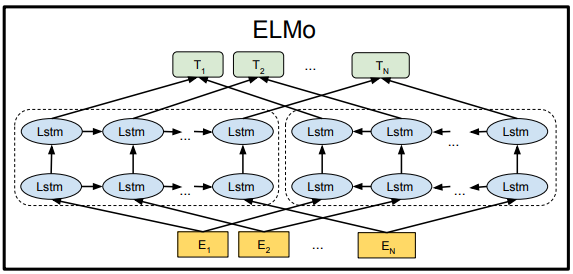
\includegraphics[scale=0.5]{picture/ELMo.png}
                \caption{ELMo}
            \end{center}
        \end{minipage}
        \hspace{1cm}
        \begin{minipage}[b]{0.5\hsize}
            \begin{center}
                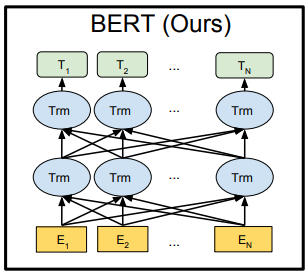
\includegraphics[scale=0.5]{picture/BERT.png}
                \caption{BERT}
            \end{center}
        \end{minipage}
    \end{tabular}
\end{figure*}

%モデルの紹介
\section{Topic and Sentiment Model with BERT}
\subsection{Topic and Sentiment Model with BERT}
本研究では、文脈を考慮できないという問題点の解決のために、文脈も学習させた分散表現を既存のトピックモデルに導入することで、その性能の向上を目指す。
本研究では、マーケティングへの応用という観点からテキストからトピックを抽出することだけでなく、センチメントの抽出も重要だと考え、分散表現を利用したセンチメントとトピックの同時抽出モデルであるTopic Sentiment Joint Model with Word Embeddings(TSWE)\cite{TSWE}に、
Word2Vecで学習された分散表現ではなくBERTで学習させた文脈を考慮した分散表現を導入することで、その性能の向上を目指す。また、文脈を考慮した分散表現の導入による性能の向上を測るべく文書レベルでの感情分類とトピック抽出による評価実験を行い、性能について検討していく。
なお、本研究で用いるパラメータは表1に示す。

TSWEにおける負の対数尤度は、$L_{k}$は以下のように設定される。
\begin{multline}
    L_{k} = \mu \parallel \nu_{k} \parallel_{2}^{2} - \\
    \displaystyle \sum_{w_{i}\in{W}} N^{k,w_{i}}\left(\nu_{k}\omega_{w_{i}} - {\rm log} \left(\displaystyle \sum_{w_{i}^{'}\in{W}} {\rm exp}(\nu_{k}\omega_{w_{i}^{'}})\right)\right)
\end{multline}

そして、L-BFGS\cite{L-BFGS}手法を適用して、$L_k$を最小化するトピックベクトル$\nu_{k}$を導出する。

\begin{table}[tbp]
    \caption{パラメータ記号とその説明}
    \centering
    \begin{tabular}{ll}
        \hline
        パラメータ            & 説明                               \\
        \hline \hline
        $D$                   & 文書数                             \\
        $d$                   & 文書インデックス                   \\
        $N$                   & 総単語数                           \\
        $N_{d}$               & 文書$d$に含まれる単語数            \\
        $V$                   & 全文書に現れる単語の種類(語彙数)   \\
        $W$                   & 文書集合                           \\
        $w_{dn} = w_{i}$      & 文書$d$に含まれる$n$番目の単語     \\
        $S$                   & センチメントのラベル数             \\
        $l$                   & センチメントラベル                 \\
        $K$                   & トピック数                         \\
        $z$                   & 割り当てられたトピック             \\
        $\nu$                 & トピックベクトル                   \\
        $\omega$              & 単語の分散表現                     \\
        $\theta$              & トピック分布                       \\
        $\phi$                & 単語分布                           \\
        $\pi$                 & センチメント分布                   \\
        $\alpha,\beta,\gamma$ & ディリクレ分布のハイパーパラメータ \\
        $s$                   & 二値指標変数                       \\
        $\lambda$             & ベルヌーイ分布のハイパーパラメータ \\
        \hline
    \end{tabular}
\end{table}

\subsection{Generative process}
本研究では、TSWEモデルを基礎とするため、改めてモデルの生成過程について以下に示す。
\begin{enumerate}
    \item For each topic-sentiment pair ($l$,$k$)
          \begin{enumerate}
              \item Genearte the word distribution of the sentiment-topic pair $\phi_{l,k} \sim $ Dir($\beta$)
          \end{enumerate}
    \item For each document $d$
          \begin{enumerate}
              \item Draw a distribution $\pi_{d} \sim $ Dir($\gamma$)
              \item For $l=1$ to $S$ under document $d$
                    \begin{enumerate}
                        \item Draw a topic distribution \\ $ \theta_{d,l} \sim $ Dir($\alpha$)
                    \end{enumerate}
              \item For each word index n from 1 to $N_{d}$
                    \begin{enumerate}
                        \item Draw a sentiment label \\ $ l_{dn}  \sim$ Multi($\pi_{d}$)
                        \item Draw a topic $z_{dn} \sim $ Multi($\theta_{d, l_{dn}}$)
                        \item Draw a binary indicator variable \\ $s_{dn} \sim $ Ber($\lambda$)
                        \item Draw a word \\$w_{dn}  \sim (1-s_{dn})$Multi$(\phi_{z_{dn},l_{dn}})+(1 - s_{dn})MulT(\nu_{z_{dn}}\omega^{\mathrm{T}}$)
                    \end{enumerate}
          \end{enumerate}
\end{enumerate}
なお、$MulT$の定義は式(1)に示している。
\subsection{Gibbs sampling}
事後分布を解析的に求めることは困難であるため、ギブスサンプリングを用いて事後分布を推定していく。サンプリングに必要な条件付確率は以下の通りである。
\begin{multline}
    P(z_{i} = k,l_{i} = l| w, z^{\neg{i}}, l^{\neg{i}}, \alpha, \beta, \gamma, \lambda, \nu, \omega) \propto
    \\ \left((1-\lambda) \cdot \frac{N_{l,k,w_{i}}^{\neg{i}} + \beta}{N_{l,k}^{\neg{i}} + V\beta} + \lambda \cdot MulT(w_{i}|\nu_{k}\omega^{\mathrm{T}})\right)
    \\ \cdot \frac{N_{d,l,k}^{\neg{i}} + \alpha}{N_{d,l}^{\neg{i}} + K\alpha} \cdot \frac{N_{d,l}^{\neg{i}} + \gamma}{N_{d}^{\neg{i}} + S\gamma}
\end{multline}
また、推定に用いられるパラメータ$\pi,\theta,\phi$は、式(4),(5),(6)で示される。
\begin{equation}
    \pi_{d,l} = \frac{N_{d,l} + \gamma}{N_{d} + S\gamma}
\end{equation}
\begin{equation}
    \theta_{d,l,k} = \frac{N_{d,l,k} + \alpha}{N_{d,l} + K\alpha}
\end{equation}
\begin{equation}
    \phi_{l,k,i} = (1-\lambda) \cdot \frac{N_{l,k,w_{i}}^{\neg{i}} + \beta}{N_{l,k}^{\neg{i}} + V\beta} + \lambda \cdot MulT(w_{i}|\nu_{k}\omega^{\mathrm{T}})
\end{equation}

%実験&検証
\section{Experiments}
本節では、文脈を考慮した分散表現の導入による性能の向上を測るべく、文書レベルでの感情分類とトピック抽出による評価実験を行い、性能について検討していく。
\subsection{Experimental setup}
\subsubsection{Using Word Embeddings}
本研究では、分散表現としてWord2Vec\footnotetext[2]{https://code.google.com/archive/p/word2vec/}とBERT\footnotetext[3]{https://github.com/google-research/bert}のオープンソースを利用する。
これらのモデルは、大規模コーパスに対して学習させる場合、時間とコストが非常にかかるためこれらの事前学習済みのモデルを利用する。

\subsubsection{Experimental datasets}
本研究では、感情分類用のデータセットとしてLarge Movie Review dataset(IMDbデータセット)\cite{IMDb}と呼ばれる大規模な映画レビューのデータセットを利用する。
このデータセットは、ポジティブかネガティブかの二値分類用データで、2万5千件の訓練用データと2万5千件のテスト用データの合計5万件のデータで構成されている。
データの前処理として、アルファベット以外の文字は削除し、アルファベットはすべて小文字にする処理も行う。加えて、
TSWEモデルに倣い、学習済み分散表現に出現しない単語や出現頻度が2以下または15以上の単語は、ストップワードとして学習には使用しない。また、コピーされたと思われるような繰り返されたレビューについても同様に削除する。
\subsubsection{Hyper Parameter Settings}
事前分布のハイパーパラメータ$\alpha, \beta, \gamma$は、TSWEモデルに倣い以下のように設定する。
\begin{equation}
    \alpha = \frac{50}{K}
\end{equation}
\begin{equation}
    \beta = 0.05
\end{equation}
\begin{equation}
    \gamma = \frac{0.05A}{S}
\end{equation}
なお、$A$は平均的な文書長とする。
\subsubsection{Evaluate Metrics}
感情分類の評価指標としては、先行研究\cite{JST,TSWE}で用いられているAccuracyを利用する。Accuracyは、分類問題で一般的に用いられることの多い評価指標である。定義については、以下の式(10)に示す。
\begin{equation}
    Accuracy = \frac{TP + TN}{TP + TN + FP + FN}
\end{equation}
なお、$TP$ = True Positive, $TN$ = True Negative, $FP$ = False Positive, $FN$ = False Negativeである。

次に、トピック抽出の評価指標としては、perplexityと自己相互情報量(PMI)を利用する。perplexityは、言語モデルの評価指標として良く用いられる指標で、言語モデルの複雑さを表す。
PMIは、Newmanら\cite{PMI}によって提案されたトピックの意味的拘束性を表す指標である。perplexityとPMIについて、以下の式(11),(12)で示す。
\begin{equation}
    {\rm perplexity} = {\rm exp}\left(-\frac{\sum_{d=1}^{D}{\rm log}p(w_{d})}{\sum_{d=1}^{D}N_{d}} \right)
\end{equation}
\begin{equation}
    {\rm PMI}(w_{i},w_{j}) = {\rm log} \frac{p(w_{i},w_{j})}{p(w_{i})p(w_{j})}
\end{equation}

\subsection{Experimental Results and Analysis}
本来なら、感情分類の結果およびトピック抽出の実験結果を載せ、それらについて考察、検討するところではあるが、実験の進捗が芳しくないためデータの記述統計の結果の図6~9に載せ、そちらについて少し言及していく。
図6は、レビュー文内の文字数についての統計である。これを見るに、0から1000文字以内の比較的短いレビュー文がレビュー全体でも多いことが分かる。全体を通して、Good/Badに大きな差は見られないと思われる。
図7は、各レビュー文内の単語数についての統計である。これを見るに、0から100単語以内の比較的短いレビューが多いことが分かる。全体を通して、Good/Badに大きな差は見られないと思われるが、0から100単語以内のレビューにおいては肯定的のレビューより否定的なレビューのほうが若干単語数が多いことが分かる。
これは、否定的な意見のほうが追求したいポイントが明確なためだと思われる。
図8は、一般的なストップワードを除いた頻出単語の上位20単語を示したものである。これを見るに、映画のレビューということもあり、1位2位には、映画に関連する単語が上がっている。
しかしながら、その他の単語を見ると何かのトピックに限定されるような単語ではないことが分かる。したがって、ストップワードの調整に関しては非常に重要だと思われる。
図9は、各テキストにおける平均単語長についての統計である。これを見るに、平均単語長は、6ぐらいであることがわかる。全体を通して、Good/Badに大きな差は見られないと思われる。

\begin{figure*}
    \begin{tabular}{cr}
        \begin{minipage}[b]{0.5\hsize}
            \begin{center}
                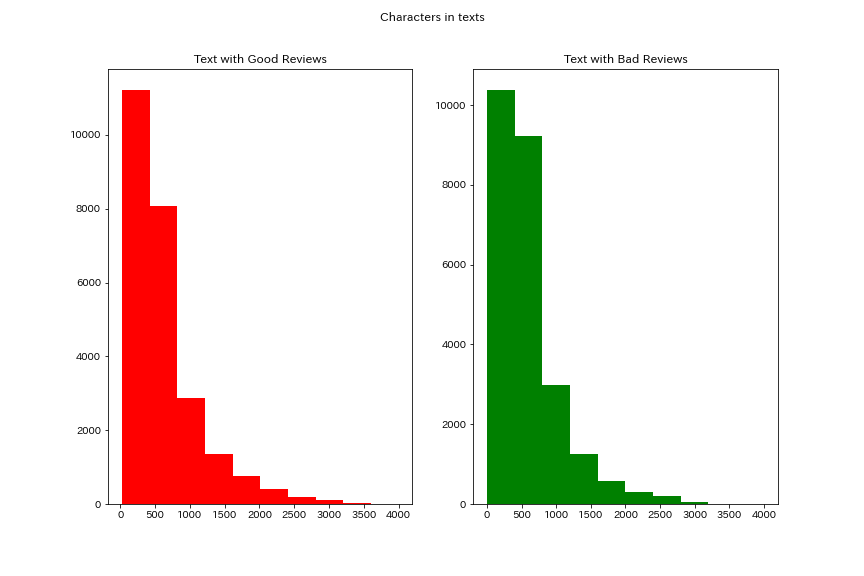
\includegraphics[width=6cm]{picture/Characters_in_texts.png}
                \caption{Number of characters in texts}
            \end{center}
        \end{minipage}
        \hspace{1cm}
        \begin{minipage}[b]{0.5\hsize}
            \begin{center}
                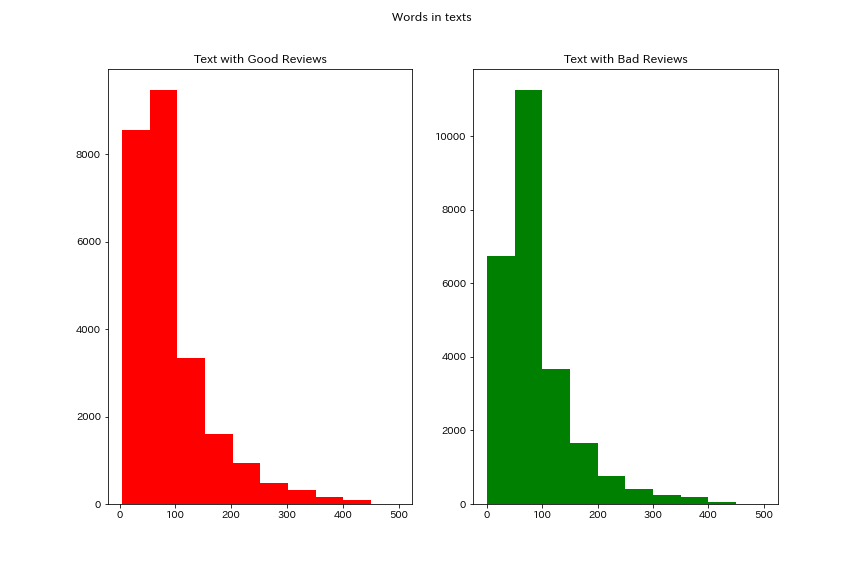
\includegraphics[width=6cm]{picture/Num_of_words_in_each_text.png}
                \caption{Number of words in each text}
            \end{center}
        \end{minipage}
    \end{tabular}
\end{figure*}
\begin{figure}[th]
    \begin{center}
        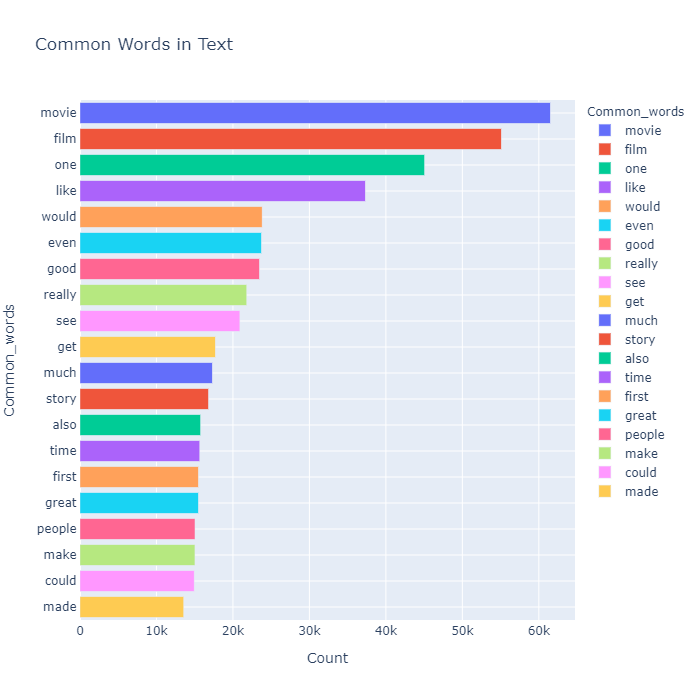
\includegraphics[width=8cm]{picture/Common_words_in_text.png}
    \end{center}
    \caption{Common Words in Text}
\end{figure}
\begin{figure*}
    \begin{center}
        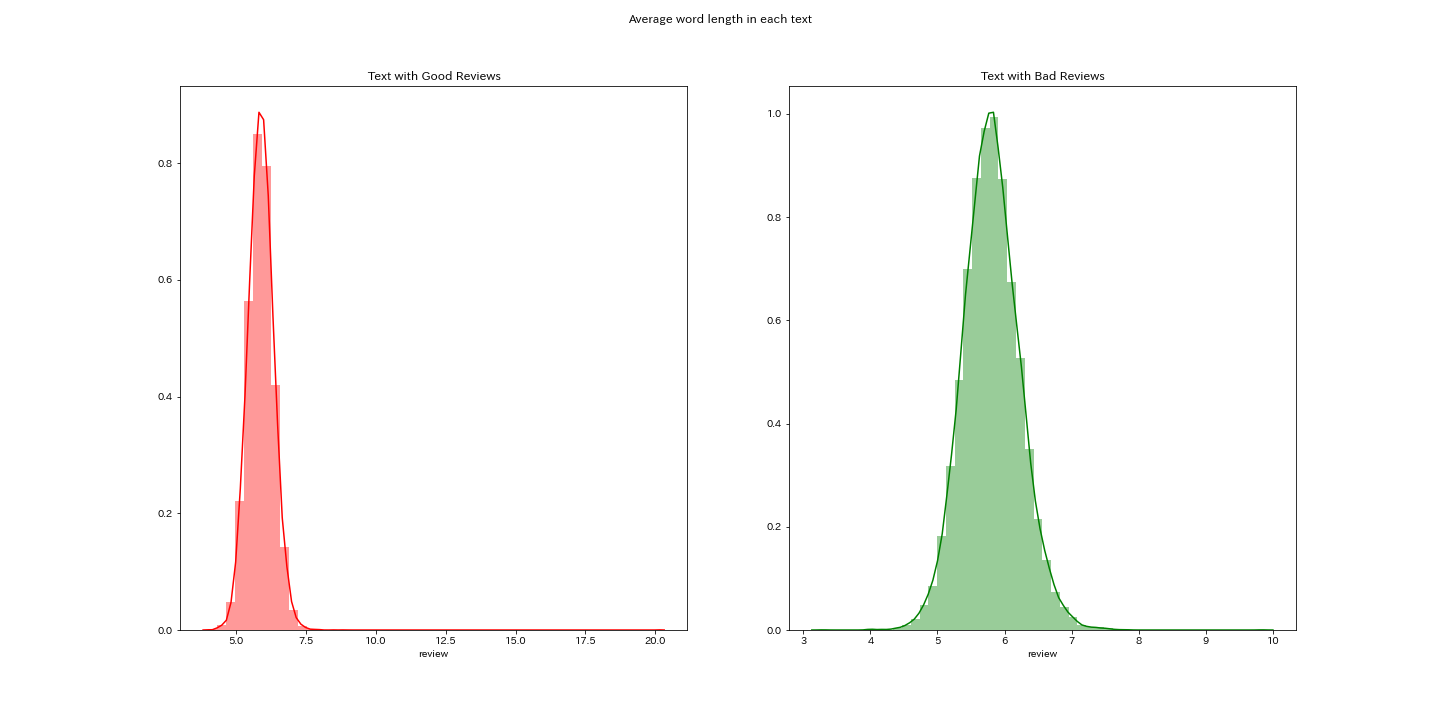
\includegraphics[width=8cm]{picture/Average_word_length_in_a_text.png}
    \end{center}
    \caption{Average word length in each text}
\end{figure*}

%結論
\section{Conclusions and Future Work}
本研究では、文脈を考慮できていないというこれまでの自然言語処理タスクにおける問題点を解決した分散表現モデルを既存のトピックモデルに導入することでその性能の向上を目的とした以下の実験を行う予定であった。
センチメントとトピックの同時抽出モデルに分散表現を取り入れたモデルに対して、文脈が考慮された分散表現を生成できる手法BERTを導入することで、感情分類の精度向上と、トピック内の意味的拘束性の向上について実験により検証していく予定である。
しかしながら、実験コードの作成に少々時間がかかってしまったため、本格的な実験には入ることができなかった。したがって、今後は実際の実験を通してモデルの性能が向上するかどうかを検証していきたい。

%\section*{謝辞}
%本研究を進めるにあたり、指導教官である東北大学大学院経済学研究科 石垣 司准教授からは多大な助言を賜りました。この場を借りてお礼申し上げます。
\begin{thebibliography}{数字}
    \bibitem{JST} Lin, C., \& He, Y. (2009). Joint sentiment/topic model for sentiment analysis. International Conference on Information and Knowledge Management, Proceedings, 375–384.
    \bibitem{LDA} Blei, D. M., Ng, A. Y., \& Jordan, M. I. (2003). Latent Dirichlet allocation. Journal of Machine Learning Research, 3(4–5), 993–1022.
    \bibitem{Gaussian LDA} Das, R., Zaheer, M., \& Dyer, C. (2015). Gaussian LDA for topic models with word embeddings. ACL-IJCNLP 2015 - 53rd Annual Meeting of the Association for Computational Linguistics and the 7th International Joint Conference on Natural Language Processing of the Asian Federation of Natural Language Processing, Proceedings of the Conference, 1, 795–804.
    \bibitem{Gaussian} Hu, P., Liu, W., Jiang, W., \& Yang, Z. (2012). Latent topic model based on Gaussian-LDA for audio retrieval. Communications in Computer and Information Science, 321 CCIS, 556–563.
    \bibitem{TSWE} Fu, X., Wu, H., \& Cui, L. (2016). Topic sentiment joint model with word embeddings. CEUR Workshop Proceedings, 1646, 41–48.
    \bibitem{Word2Vec} Mikolov, T., Sutskever, I., Chen, K., Corrado, G., \& Dean, J. (2013). Distributed representations of words and phrases and their compositionality. Advances in Neural Information Processing Systems, 1–9.
    \bibitem{ELMo} Peters, M. E., Neumann, M., Iyyer, M., Gardner, M., Clark, C., Lee, K., \& Zettlemoyer, L. (2018). Deep contextualized word representations. NAACL HLT 2018 - 2018 Conference of the North American Chapter of the Association for Computational Linguistics: Human Language Technologies - Proceedings of the Conference, 1, 2227–2237.
    \bibitem{BERT} Devlin, J., Chang, M. W., Lee, K., \& Toutanova, K. (2019). BERT: Pre-training of deep bidirectional transformers for language understanding. In NAACL HLT 2019 - 2019 Conference of the North American Chapter of the Association for Computational Linguistics: Human Language Technologies - Proceedings of the Conference (Vol. 1).
    \bibitem{LSI} Landauer, T. K., \& Dumais, S. T. (1997). A solution to Plato's problem: The latent semantic analysis theory of acquisition, induction, and representation of knowledge. Psychological Review, 104(2), 211–240.
    \bibitem{pLSI} Hofmann, T. (1999). Probabilistic latent semantic indexing. Proceedings of the 22nd Annual International ACM SIGIR Conference on Research and Development in Information Retrieval, SIGIR 1999, 51(2), 50–57.
    \bibitem{Graph} Tutubalina, Elena \& Nikolenko, Sergey. (2017). Demographic Prediction Based on User Reviews about Medications. Computacion y Sistemas. 21. 227-241. 10.13053/CyS-21-2-2736.
    \bibitem{LSTM} Hochreiter, S. and Schmidhuber, J. (1997). Long Short-Term Memory, Neural Computation, Vol. 9, No. 8, 1735–1780
    \bibitem{Transformer} Vaswani, A., Shazeer, N., Parmar, N., Uszkoreit, J., Jones, L., Gomez, A. N., Kaiser, Ł., \& Polosukhin, I. (2017). Attention is all you need. Advances in Neural Information Processing Systems, 2017-December(Nips), 5999–6009.
    \bibitem{L-BFGS} Liu, D. C., \& Nocedal, J. (1989). On the limited memory BFGS method for large scale optimization. In Mathematical Programming, (Vol. 45), 503-528.
    \bibitem{IMDb} Andrew L. Maas, Raymond E. Daly, Peter T. Pham, Dan Huang, Andrew Y. Ng, and Christopher Potts. (2011). Learning Word Vectors for Sentiment Analysis. The 49th Annual Meeting of the Association for Computational Linguistics (ACL 2011)
    \bibitem{PMI} David Newman, Sarvnaz Karimi, and Lawrence Cavedon.(2009) External evaluation of topic models. pages 11-18, December.
\end{thebibliography}
\end{document}
